\documentclass[10pt, conference]{IEEEtran}
\usepackage{graphicx}
\usepackage{amsmath}
\usepackage{amssymb}
\usepackage{gensymb}
\usepackage{float}
% \usepackage[labelfont=bf]{caption}

\usepackage{listings}
\usepackage{textcomp}
\usepackage[usenames,dvipsnames]{color} 
\usepackage{courier}
\definecolor{mygrey}{gray}{.96} % Light Grey
\lstset{ 
	language=verilog,              % choose the language of the code ("language=Verilog" is popular as well)
   tabsize=4,							  % sets the size of the tabs in spaces (1 Tab is replaced with 3 spaces)
	basicstyle=\footnotesize\ttfamily, % the size of the fonts that are used for the code
	% numbers=left,                   % where to put the line-numbers
	% numberstyle=\tiny,              % the size of the fonts that are used for the line-numbers
	% stepnumber=1,                   % the step between two line-numbers. If it's 1 each line will be numbered
	% numbersep=5pt,                  % how far the line-numbers are from the code
	backgroundcolor=\color{mygrey}, % choose the background color. You must add \usepackage{color}
	%showspaces=false,              % show spaces adding particular underscores
	%showstringspaces=false,        % underline spaces within strings
	%showtabs=false,                % show tabs within strings adding particular underscores
	frame=single,	                 % adds a frame around the code
	tabsize=3,	                    % sets default tabsize to 2 spaces
	captionpos=b,                   % sets the caption-position to bottom
	breaklines=true,                % sets automatic line breaking
	breakatwhitespace=false,        % sets if automatic breaks should only happen at whitespace
	%escapeinside={\%*}{*)},        % if you want to add a comment within your code
	commentstyle=\color{BrickRed}   % sets the comment style
}


%
% Title.
\title{EE230: Project Simulation Report\\
Sound Localization Circuit}

% Author
\author{Sarthak Consul --- 16D100012\\
        Tushar Dhawal Baranwal --- 16D100009}

\begin{document}
\IEEEoverridecommandlockouts
\IEEEpubid{\makebox[\columnwidth]{}
\hspace{\columnsep}\makebox[\columnwidth]{ }}

\maketitle

% \begin{abstract}
% We make an analog circuit that calculates the phase difference between two sinusoids of the same frequency. This circuit is then used to locate a distant sound source. Two receivers placed slightly away from one another receive a sinusoidal waveform generated by a sound source. The phase difference between the two waves is computed by our analog circuit, which gives an estimate of the direction the sound wave is coming from. This is much simpler and faster than the existing methods. 
% \end{abstract}

\section{INTRODUCTION}
We plan to implement a circuit that is able to accurately locate a distant sound source. The circuit design is inspired by the biaural hearing mechanism found in nature.\\
The papers \cite{1031521} - \cite{541607} are used as a guidelines for the circuit design.

% \IEEEpubidadjcol

\section{OVERVIEW OF OUR ARCHITECTURE}
The audio frequency used to detect the source is chosen to be 5kHz (or a narrow bandpass filter could be used to extract this frequency component). The circuit is setup as follows: There are two microphones placed slightly apart. This results in a difference in the distance covered by the signal from the source to the 2 microphones. (This difference in path does not result in significant amplitude difference). This results in a phase shift that, if measured, is directly correlated to the location of the source (more accurately its spatial angle/ direction).

\begin{figure}[hbp]
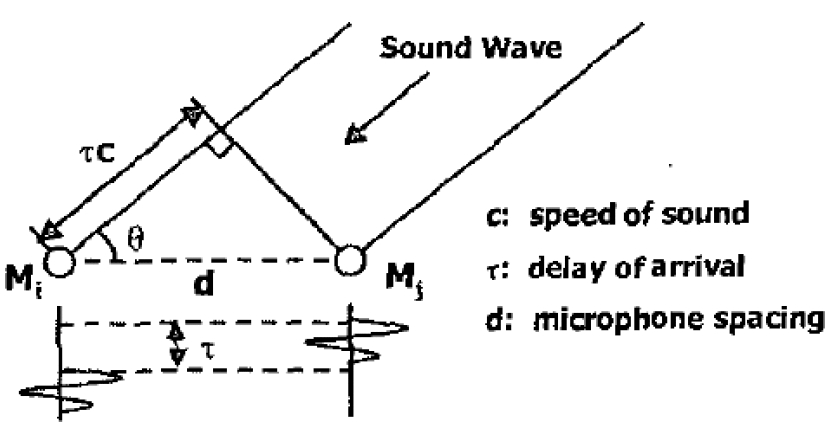
\includegraphics[width=\columnwidth]{SpatialAngle.jpg}
\caption{Path Difference due to spatial angle of source. Taken from \cite{1031521}}
\label{fig:spatial_angle}
\end{figure}

\begin{equation*}
    \text{Delay, }\tau = \frac{d\cos{\theta}}{c}\\
    \text{Phase difference }= \frac{2\pi f d\cos{\theta} }{c}
\end{equation*}

One of the 2 signals (say $V_1$) is used as a reference signal while the other (say $V_2$) is delayed until its phase is roughly the same as that of the reference. This is done by having a voltage controlled resistance in the delay circuit, and having the tuning voltage be varied via a feedback mechanism.
\begin{figure}[hbp]
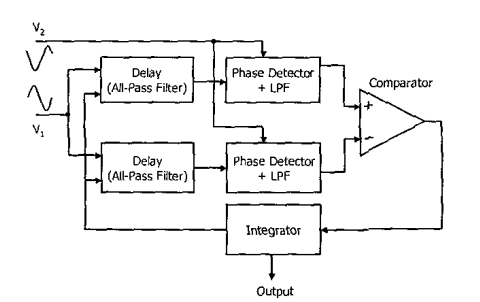
\includegraphics[width=\columnwidth]{block_cir.PNG}
\caption{The figure gives the Block Diagram of the sound locator circuit}
\label{fig:block_cir}
\end{figure}
The feedback mechanism consists of the phase detector block followed by a comparator and an integrator.

% \begin{figure}[hbp]
% 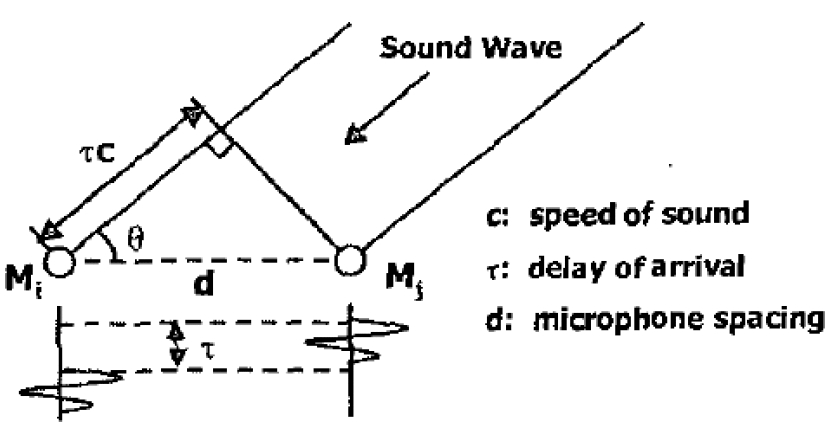
\includegraphics[width=\columnwidth]{SpatialAngle.jpg}
% \caption{Path Difference due to spatial angle of source. Taken from \cite{1031521}}
% \label{fig:spatial_angle}
% \end{figure}


\section{SIMULATION SETUP}
Simulation is done using Ngspice. Model files for components were obtained either from the WEL Lab or porting PSpice files obtained from TINA-TI\textsuperscript{TM} \small{TINA-TI is a SPICE based Analog Simulation Program developed by DesignSoft in collaboration with Texas Instruments}\normalsize to Ngspice.\\
Each block (see Figure~\ref{fig:block_cir}), is separately simulated and analyzed. Complete analysis of circuit is done in Section V.

\subsection{SIMULATION OF DELAY CIRCUIT}
The delay circuit is essentially an all-pass filter.
The phase difference introduced depends on the resistance $R_{ph}$, which should be controlled by a tuning voltage, $V_T$.

\begin{figure}[H]
    \centering
    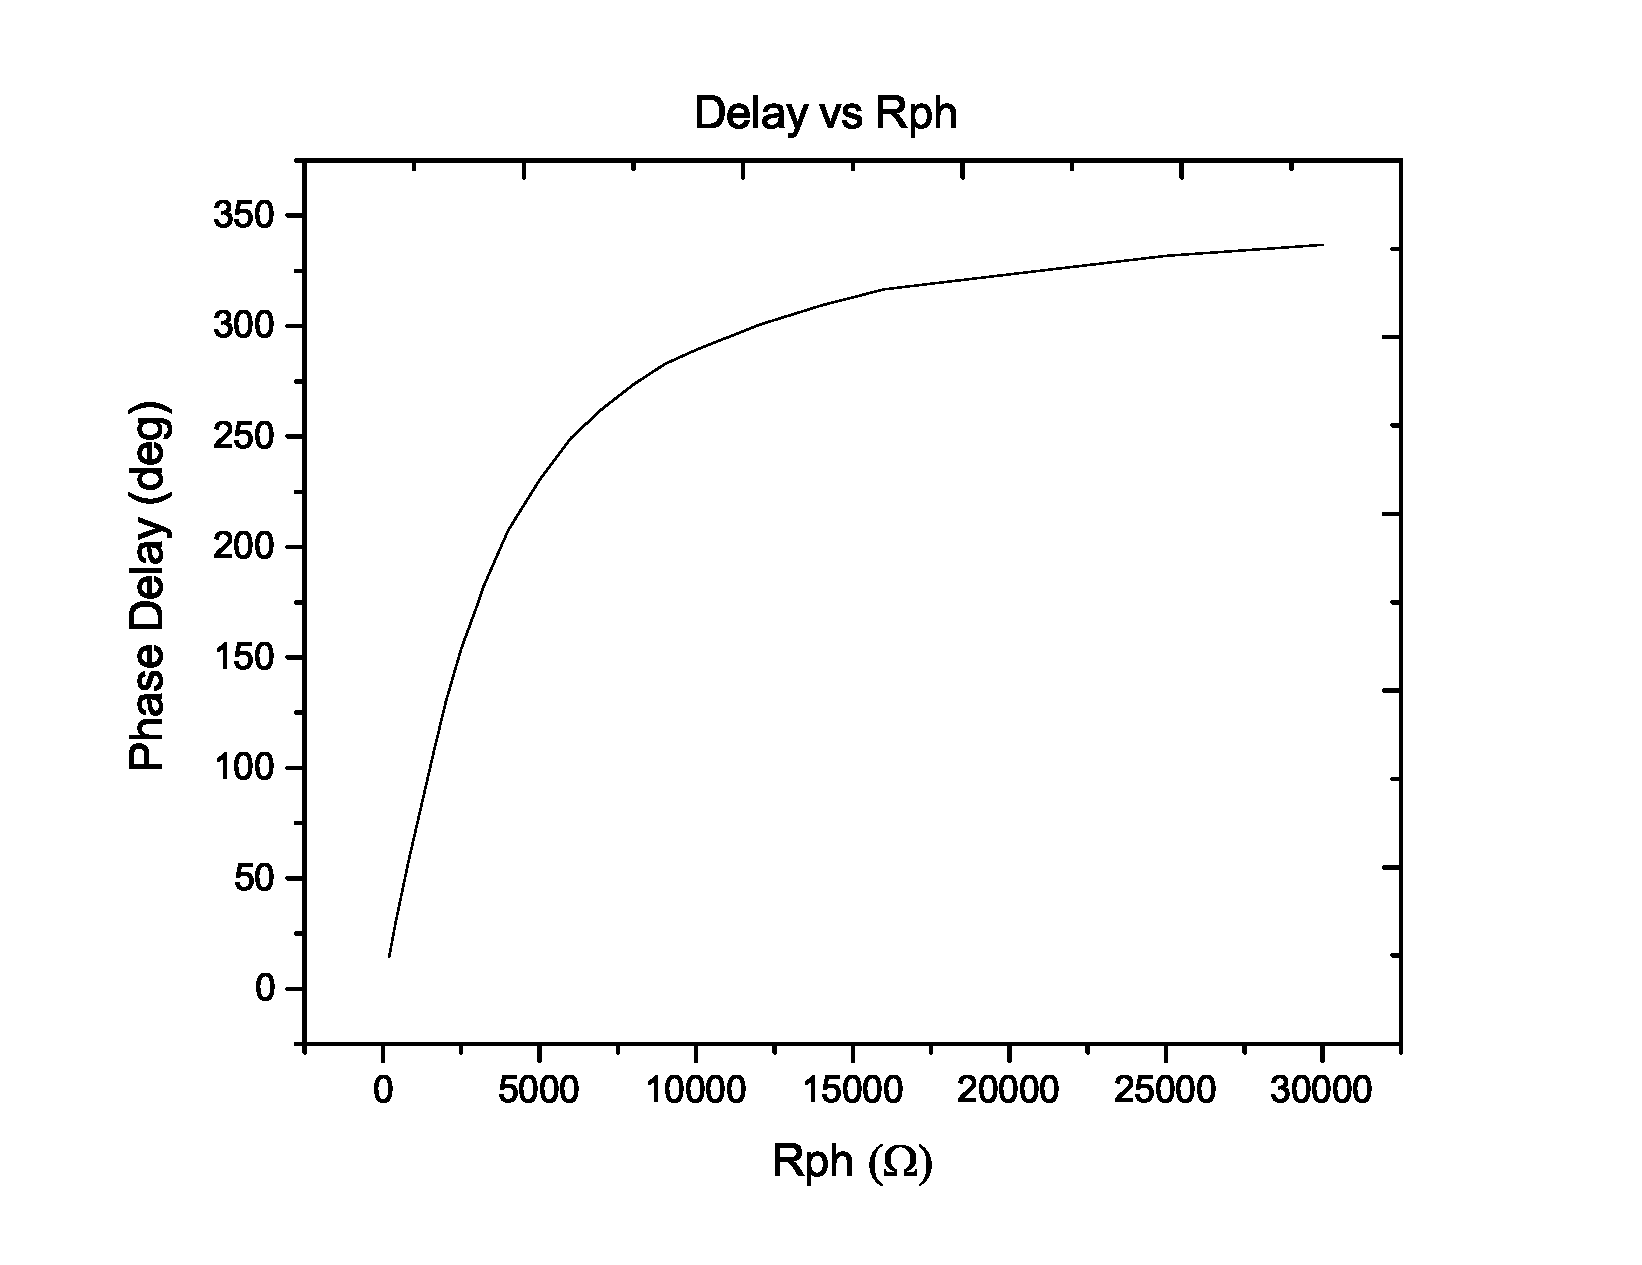
\includegraphics[width=\columnwidth]{Delay_vs_Rph.eps}
    \caption{Variation of Phase delay with change in $R_{ph}$}
    \label{fig:delay_vs_Rph}
\end{figure}

To achieve the desired range of phase difference of $20\degree$ to $350\degree$, $R_{ph}$ must be varied by a range of around 2 decades.
The voltage controlled resistance can be realized by
\begin{itemize}
    \item using a JFET (BFW10) with the tuning voltage as its gate voltage.\\
    or
    \item LM13700 IC
\end{itemize}

We have decided to use the JFET approach due to its convenience and the fact that, exploiting subthreshold conduction (where resistance varies exponentially). we are able to vary $R_{DS}$ by the required range 2 decades.

\begin{figure}[bhp]
    \centering
    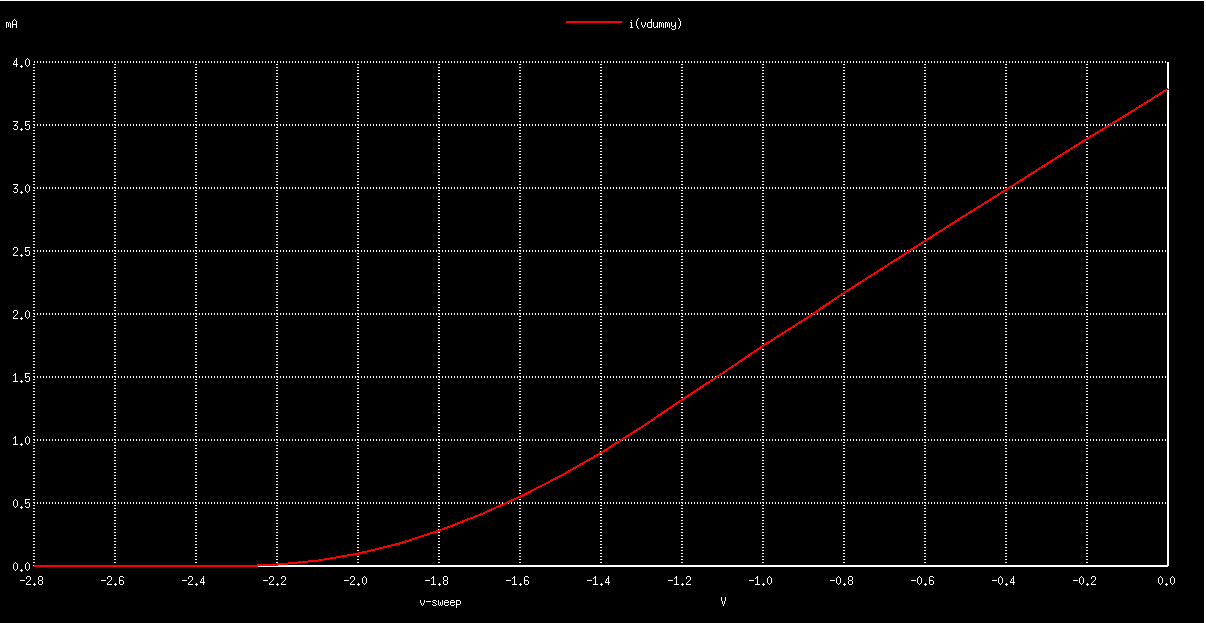
\includegraphics[width=\columnwidth]{GIT_Id_vs_Vgs.PNG}
    \caption{$I_d$ vs. $V_{GS}$ curve of BFW10}
    \label{fig:Id_Vgs}
\end{figure}
The simulation (Figure~\ref{fig:Id_Vgs}) indicates that the threshold voltage of the FET is around -1.8V while the cut-off voltage is approximately 2.25V.

From Table~\ref{tab:Rds_vs_Vgs}, it is clear that the the JFET's drain to source resistance has the suitable variation when $V_{GS}$ is kept between -2.3V to 0.6V \footnote{actual range has to be determined from practical testing}. Also by plotting this, (see Figure~\ref{fig:rds_vs_vgs}) it is a greater source-drain resistance is offered by the FET when $V_{GS}$ is more negative.

\begin{figure}[htbp]
    \centering
    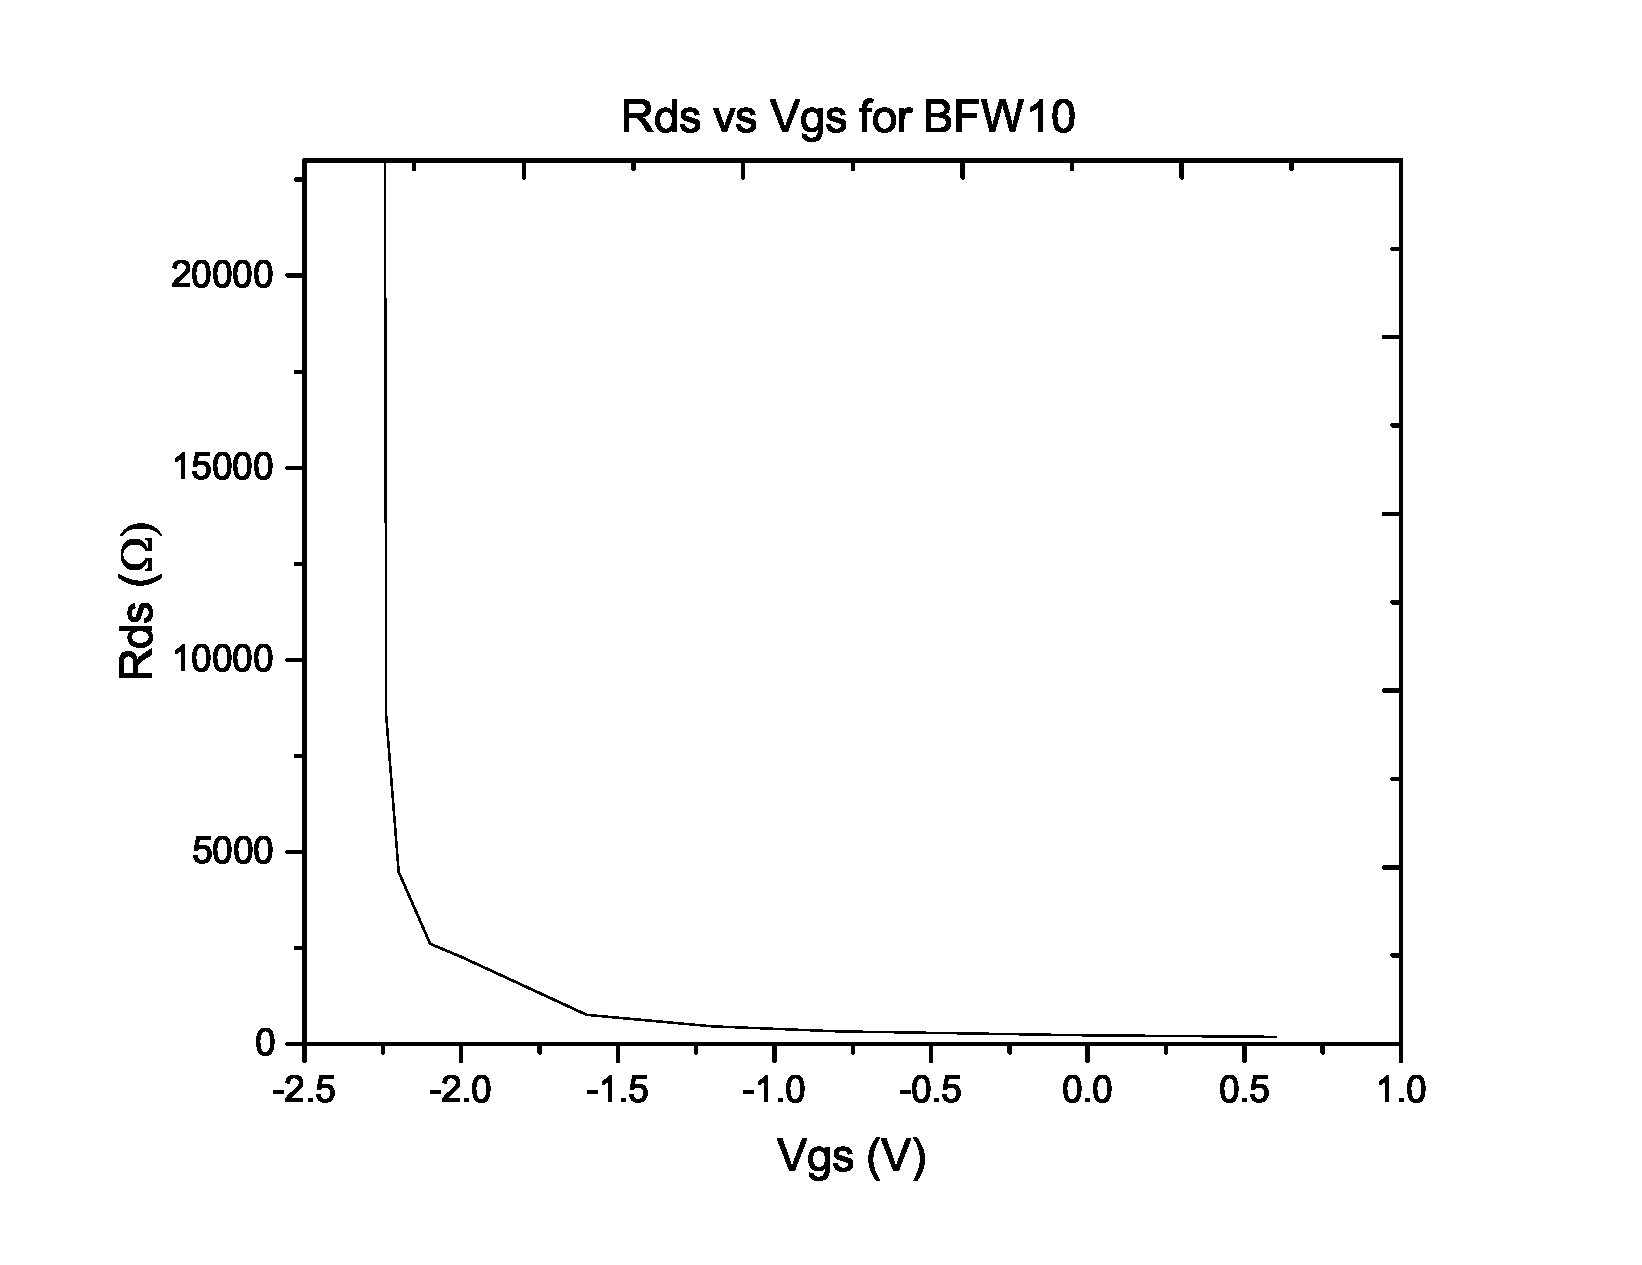
\includegraphics[width=\columnwidth]{rds_vs_vgs.eps}
    \caption{$R_{DS}$ vs. $V_{GS}$ for BFW10}
    \label{fig:rds_vs_vgs}
\end{figure}

\begin{figure}[htbp]
    \centering
    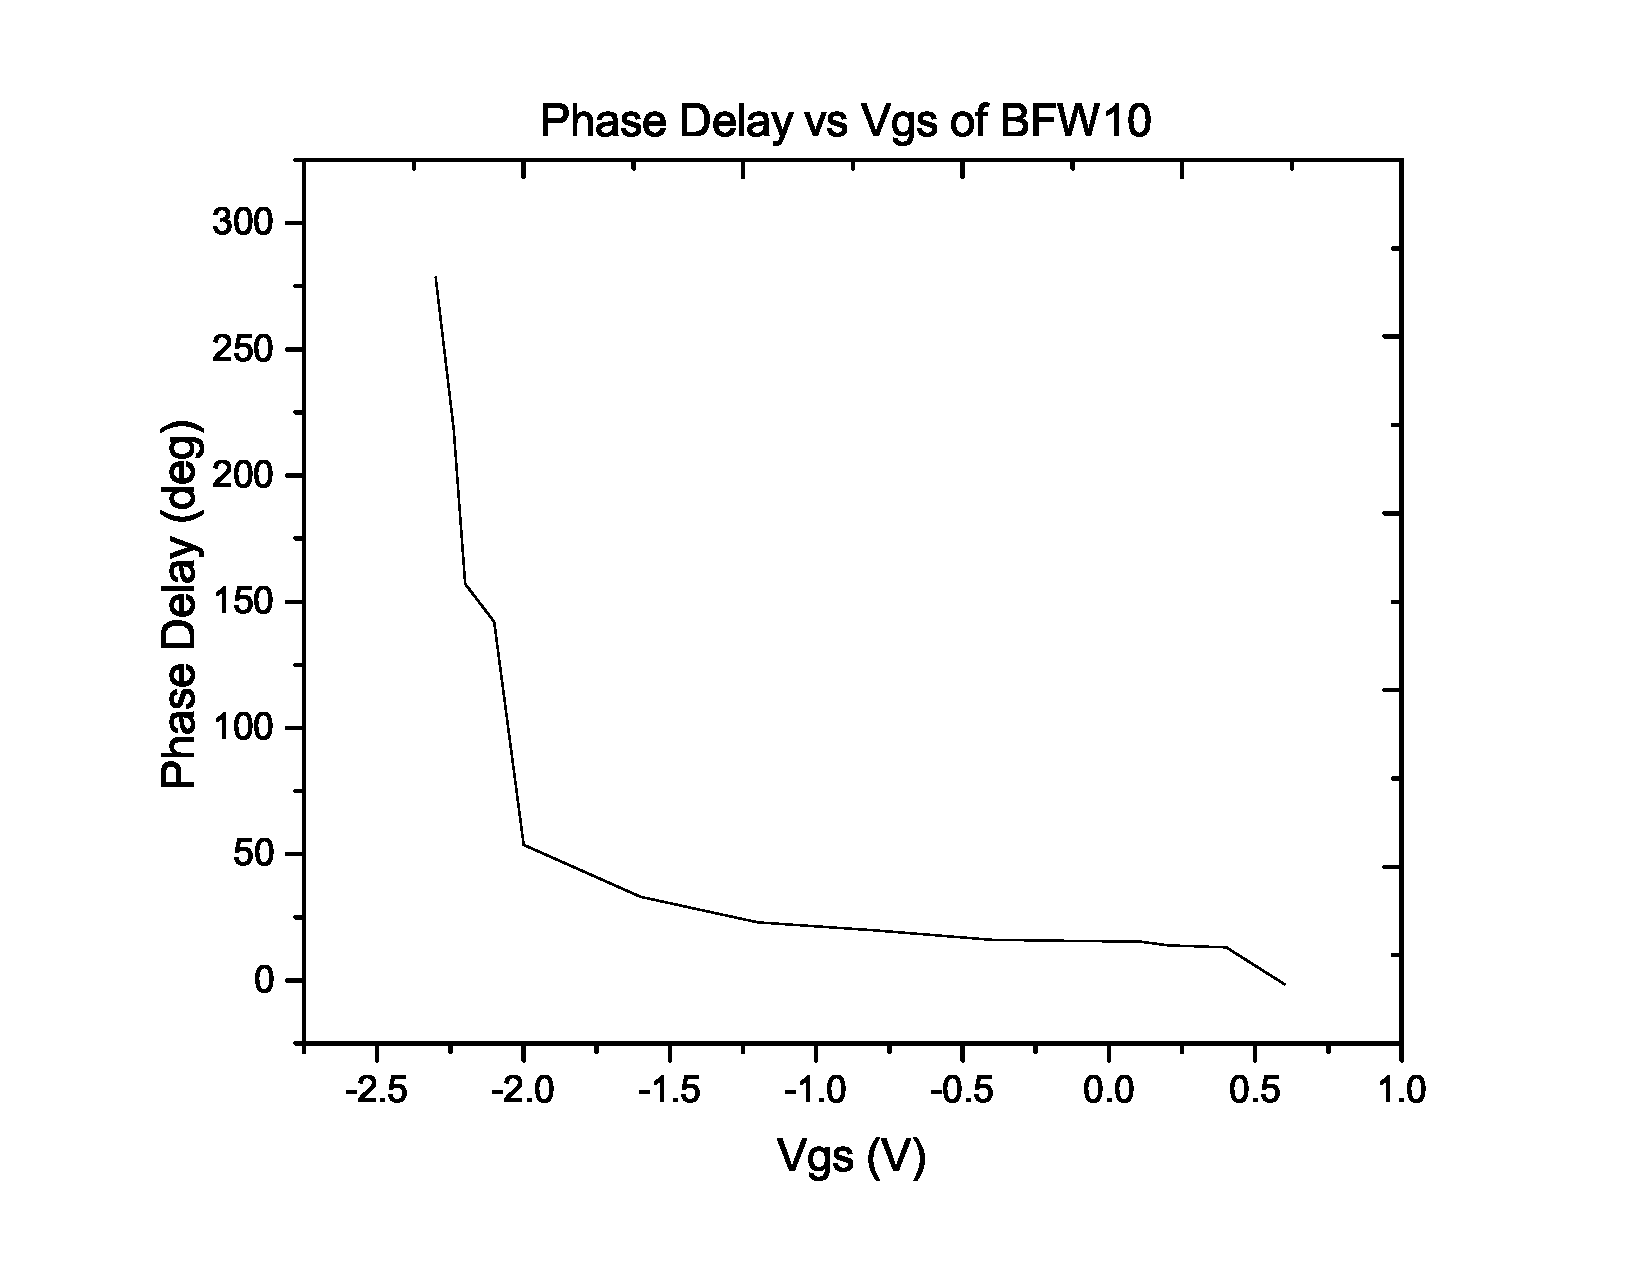
\includegraphics[width=\columnwidth]{Delay_vs_VT.eps}
    \caption{Delay vs. $V_{GS}$ for BFW10}
    \label{fig:rds_vs_VT}
\end{figure}

Figure~\ref{fig:rds_vs_VT}  sugests that the DC value of $V_{GS}$ of the JFET is approximately linearly related to the phase delay introduced by the delay circuit (for the range of $50\degree \leq \Delta \phi \leq 360\degree$. Thus from the steady state \footnote{\cite{1031521} suggests that this would occur within 1ms} value of $V_{T-DC}$, the phase difference of the 2 signals and so the spatial direction of the source can be determined.


\subsection{SIMULATION OF PHASE DETECTOR}
The goal of this block is to get the phase difference  between 2 signals and output a signal whose DC value should be a measure of the phase difference. There are various ways to do this, such as:
\begin{itemize}
    \item use a multiplier circuit
    \item use Zero-Cross Detector on the 2 signals, find the difference of the resulting signals and rectify (full/half) the difference 
\end{itemize}
To minimize, both the hardware cost/ complexity and delay of the circuit, the first approach is used. We plan to use the MPY634 IC. Due to the lack of model file, the sigmult model inbuilt with Spice is used in our simulations.
A multiplication factor of 10 is also introduced (by setting the Scale Factor of the MPY634 to 0.1) to ensure that the signal magnitude does not become too small.

\begin{equation*}
    A\sin{(\omega t)}\times A\sin{(\omega t +\phi)}=A^2/2[\cos{\phi} - \cos{(2\omega t + \phi)}]
\end{equation*}

\subsection{SIMULATION OF LOW PASS FILTER}
Input to the LPF is the product of 2 coherent sine waves. Its output should be the DC wave of the product.

If the cut-off frequency of the Low Pass Filter is sufficiently lesser than $2\omega =$10kHz, the output would be DC component, which is solely dependant on the phase difference of the 2 sine waves.\\
The cut-off frequency of 10.61Hz is chosen.
\begin{figure}[bhp]
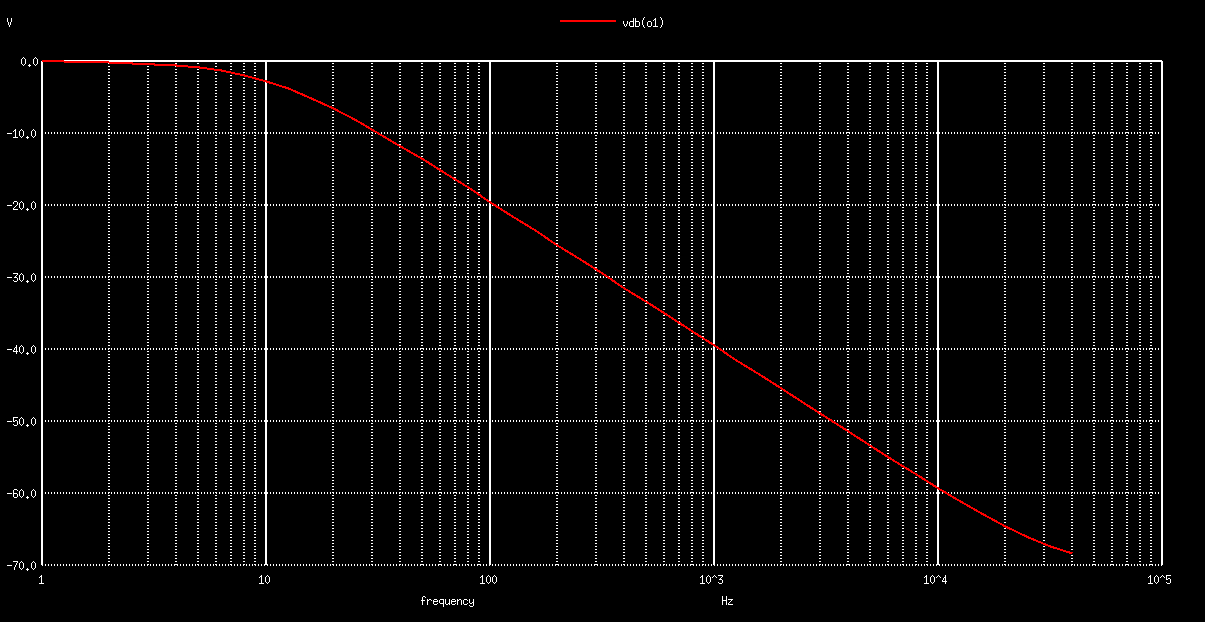
\includegraphics[width=\columnwidth]{LPF_AmpBodePlot.PNG}
\caption{Amplitude Bode Plot of Low Pass Filter}
\label{LPF_bode}
\end{figure}
It is clear that the filter will attenuate the 10kHz component by a factor of around 60dB, thereby making its output the DC component of the product.\\

The 2 DC voltages obtained from each branch are compared with a comparator (made using an Op-Amp with no feedback). For inputs will be $MA^2/2\cos{\phi_1}$ and $MA^2/2\cos{\phi_2}$ and the output would be positive when $\phi_1$ is smaller than $\phi_2$ and negative otherwise.

\subsection{SIMULATION OF INTEGRATOR}
The integrator is simply a capacitor with a resistive element as a dampening element. Limiters are used to ensure that the tuning voltage of the delay circuit is maintained within the locking range of 0.6V to $-2.3$V. 

\begin{figure}[bhp]
\centering
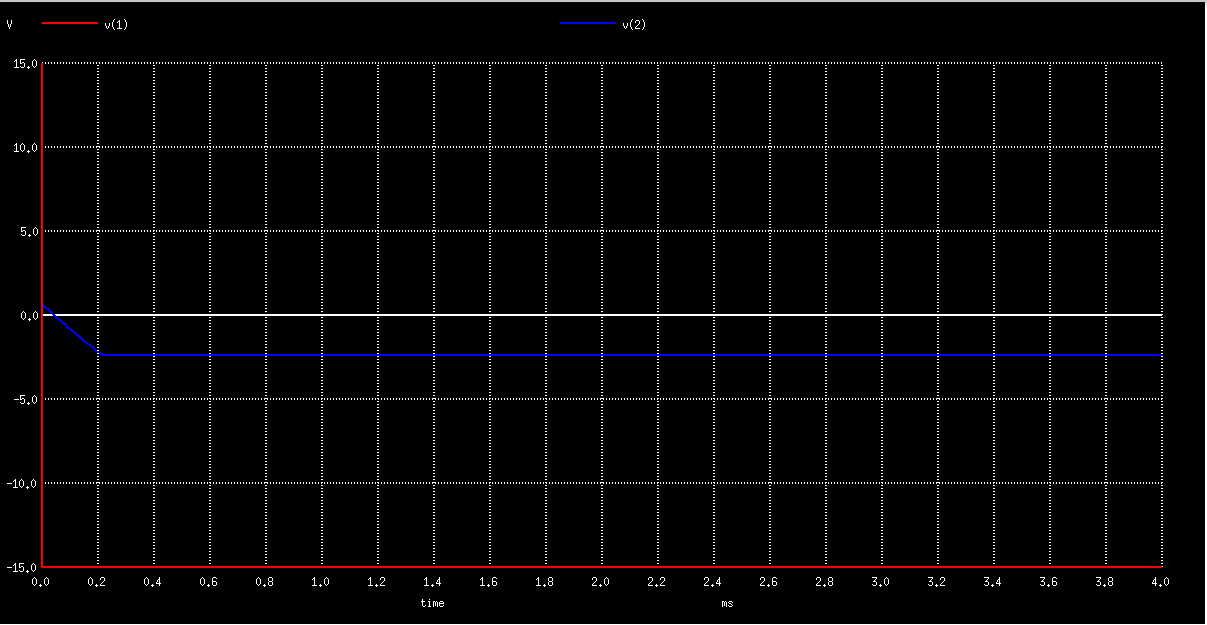
\includegraphics[width=\columnwidth]{int_Negative.PNG}
\caption{Voltage limiting at large negative dc inputs}
\label{int_neg}
\end{figure}

\begin{figure}[bhp]
\centering
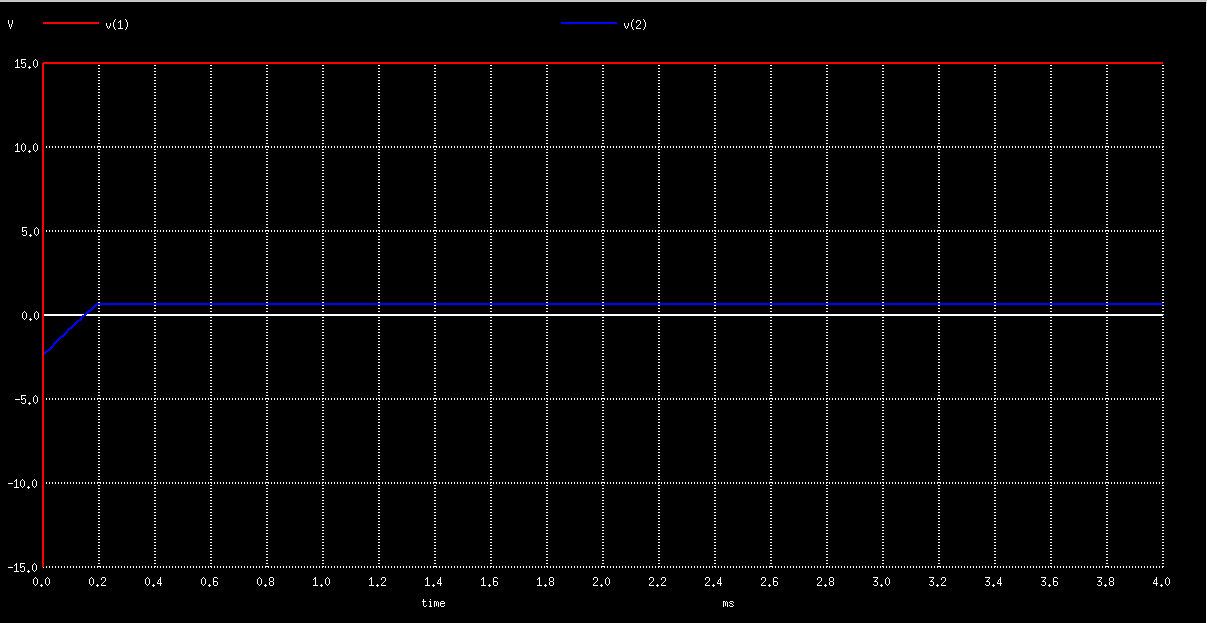
\includegraphics[width=\columnwidth]{int_Positive.PNG}
\caption{Voltage limiting at large positive dc inputs}
\label{int_pos}
\end{figure}


\section{OBSERVATIONS}
The following observations are key to understanding how the circuit operates:
\begin{itemize}
    \item [--] The BFW10 JFET is an n-channel FET, so its $R_{DS}$ value increases with reduction in $V_{GS}$. Thus the delay circuit introduces to its input increases with decrease in the dc component of tuning voltage.
   % \item [--] The \textcolor{red}{ABOUT SMALLER DELAY VS LARGER DELAY COMAPRISON}
    \item [--] A positive output of comparator will charge the capacitor (of integrator block) and so increase $V_{T-DC}$, while negative output would decrease $V_{T-DC}$.
    \item [--] Both \cite{1031521} and  \cite{541607} suggest that the there is a linear relation between DC output voltage and the input phase difference. This has been verified by figure~\ref{fig:delay_vs_VT}
\end{itemize}

\section{Analysis of the circuit as a whole}

The overall operation of the circuit is elegant and simple. From the microphones, 2 phase shifted signals are obtained. The phase difference is a function of the distance between the receivers, which is known and the direction the sound wave is coming from. Once the two signals are obtained, we need to compute the phase delay between the two signals.
For this, we use two delay circuits with slightly different time delays. Assuming both signals have the same amplitude and frequency, $V_{1}$ goes to the two delay elements and we have two versions of $V_{1}$ delayed by different time constants. Our aim is to adaptively control the different delays such that the phase of the delayed signal approaches the phase of $V_{2}$. The delay generated by our delay circuits is a function of the gate voltage applied to the MOSFET, which acts as a voltage controlled resistor, when it is operating in the triode region. 
Then the delayed signals are correlated with the original input signal and the DC outputs are fed to the comparator. The output of the comparator is fed to the delay circuit through an integrator, implemented using a capacitor. To ensure there are no large oscillations we add a damping element in the form of a resistor.
Moreover, since the inputs to the delay blocks have to vary from 0.6V to $-2.3$V, the output of the comparator was constrained to be in this region using a limiter to ensure the circuit does not go outside its locking range. The output voltage is taken from the voltage across the integrator. The phase difference can be obtained from the graph between tuning voltage and the delay generated. However, the entire circuit cannot be simulated because the capacitors cannot be given charge initially in the simulation, as is necessary. 
However, the individual parts have been simulated and tested successfully and careful analysis has been done to ensure it will work well in conjunction also. 

\bibliographystyle{unsrt}
\bibliography{research}

\appendices

\section{Simulation Code}

% 	\begin{minipage}{\columnwidth}
% 		\lstinputlisting[caption= Low Pass Filter Circuit]{LPF.cir}
% 		\label{delay_code}
% 	\end{minipage}

% 	\begin{minipage}{\columnwidth}
% 		\lstinputlisting[caption = Delay Block circuit]{delayblock.cir}
% 		\label{delayblock_code}
% 	\end{minipage}
	
% 	\begin{minipage}{\columnwidth}
% 		\lstinputlisting[caption = Integrator Ciruit]{integrator.cir}
% 		\label{integrator_code}
% 	\end{minipage}
	
		
\section{Data Tables}

\begin{table}[H]
    \centering
    \caption{($2^{nd}$ Order)Phase Shift with change in $R_{ph}$ for input signal frequency of 5kHz}
\begin{tabular}{|c|c|c|c|c|}
\hline
$R_{ph}$ & $\tau_1$ (in ms) & $\tau_2$ (in ms) & $\phi_1$  (in $\degree$) & $\phi_2$ (in $\degree$) \\ 
\hline
200 & 0.004 & 0.009 & -7.201 & -14.4 \\ 
400 & 0.009 & 0.017 & -14.4 & -30.114 \\ 
800 & 0.016 & 0.032 & -28.152 & -56.952 \\ 
1600 & 0.03 & 0.059 & -53.01 & -106.038 \\ 
2000 & 0.036 & 0.072 & -64.8 & -129.6 \\ 
2500 & 0.043 & 0.086 & -76.59 & -153.81 \\ 
3000 & 0.048 & 0.097 & -86.401 & -173.466 \\ 
3200 & 0.05 & 0.101 & -90 & -181.674 \\ 
4000 & 0.058 & 0.116 & -103.41 & -207.486 \\ 
5000 & 0.065 & 0.128 & -115.2 & -230.4 \\ 
6000 & 0.07 & 0.139 & -124.362 & -249.39 \\ 
7000 & 0.073 & 0.146 & -130.914 & -262.476 \\ 
8000 & 0.076 & 0.152 & -136.8 & -273.6 \\ 
9000 & 0.079 & 0.158 & -142.038 & -282.762 \\ 
10000 & 0.081 & 0.161 & -145.314 & -289.314 \\ 
12000 & 0.084 & 0.167 & -150.552 & -300.438 \\ 
14000 & 0.085 & 0.172 & -151.686 & -309.438 \\ 
16000 & 0.088 & 0.176 & -158.328 & -316.656 \\ 
18000 & 0.089 & 0.178 & -159.984 & -319.986 \\ 
20000 & 0.09 & 0.18 & -161.658 & -323.334 \\ 
25000 & 0.092 & 0.185 & -164.988 & -331.668 \\ 
30000 & 0.094 & 0.188 & -168.318 & -336.654 \\ 
\hline
\end{tabular}
    \label{tab:delay_vs_rph}
\end{table}

\begin{table}[H]
    \centering
    \caption{Drain to Source Resistance of BFW10 vs $V_{GS}$}
\begin{tabular}{|c|c|c|c|}
\hline
$V_{GS}$ (in V) & $R_{DS}$ (in $\Omega$) &  $2^{rd}$ Order Delay \\
\hline
0.6 & 179.909 & 12.94 \\
0.4 & 193.151 & 13.89 \\
0.2 & 213.779 & 15.37 \\
0.1 & 215.295 & 15.478 \\
0 & 223.379 & 16.057 \\
-0.4 & 275.422 & 19.782 \\
-0.8 & 318.908 & 22.886 \\
-1.2 & 460.74 & 32.945 \\
-1.6 & 759.69 & 53.694 \\
-2 & 2268.98 & 141.929 \\
-2.1 & 2599.9 & 156.966 \\
-2.2 & 4481.55 & 218.461 \\
-2.24 & 8554.52 & 278.36 \\
-2.3 & 232627 & 356.865 \\
% \multicolumn{2}{c|}{Phase Difference Possible} \\
% \cline{3-4}
%  &  & $2^{nd}$ Order Delay &
\hline
\end{tabular}
    \label{tab:Rds_vs_Vgs}
\end{table}
\end{document}